\documentclass[12pt, a4paper]{article}

\title{\textsc{Intro.~to Computer Networks}\\Lab 2 Report}
\author{110062219 翁君牧}
\date{\today}

\usepackage{xeCJK}
\usepackage{float}
\usepackage{amsmath}
\usepackage{amssymb}
\usepackage{caption}
\usepackage{subcaption}
\usepackage{tikz}
\usepackage{pgfplots}
\usepackage{listings}
\usepackage{hyperref}
\usepackage{booktabs}
\usepackage{inputenc}
%\usepackage{biblatex}
\usepackage{longtable}

\setCJKmainfont{Songti TC}
\setCJKsansfont{Heiti TC}

\newfontface\ccpl{Cascadia Code PL}

\lstset{
	breaklines=true,
	basicstyle=\ttfamily,
}

\definecolor{nthu}{HTML}{7F1084}

\begin{document}

\maketitle

\tableofcontents

\section{建置與測試}

上傳至 eeclass 的版本共計有 v0, v1 二個,分別為 Basic 及  Bonus, 接下來主要以後者為主。使用 \texttt{unzip} 指令解壓縮後,將得到一個目錄,切換為 working directory, 當中包含以下內容:

\begin{description}
\item[\ttfamily README.pdf] 即本 report.
\item[\ttfamily Makefile] 詳見以下說明。
\item[\ttfamily src/] Server, client 的原始碼。
\item[\ttfamily include/] 兩者共用的 header, 包括 packet 的 declarations, sliding window 和 buffer 的大小以及我慣用的 macros.
\item[\ttfamily test/] 測試用的 shell script 與檔案。
\end{description}

\texttt{Makefile} 預設將以 \texttt{gcc} 編譯 \texttt{src/} 下所有 \texttt{*.c} files 為 binary files 至 \texttt{bin/} 中。與上次相同,另外還提供兩種 targets \textsf{nevikw39}, \textsf{debug}. 前者在編譯時期將有更多警告以及提示訊息,後者則更會在執行時期於 \texttt{stderr} 以黃字輸出偵錯訊息並檢查越界存取、undefined behaviors 等。

至於測試的部分,我寫了一份 script 作為 Makefile 的 \textsf{test} target, 首先複製一些檔案,接著執行 server 並置於背景,然後執行 client 下載一些檔案,最後檢查下載下來的檔案是否與原本的完全一致。

\begin{figure}[htbp]
\centering
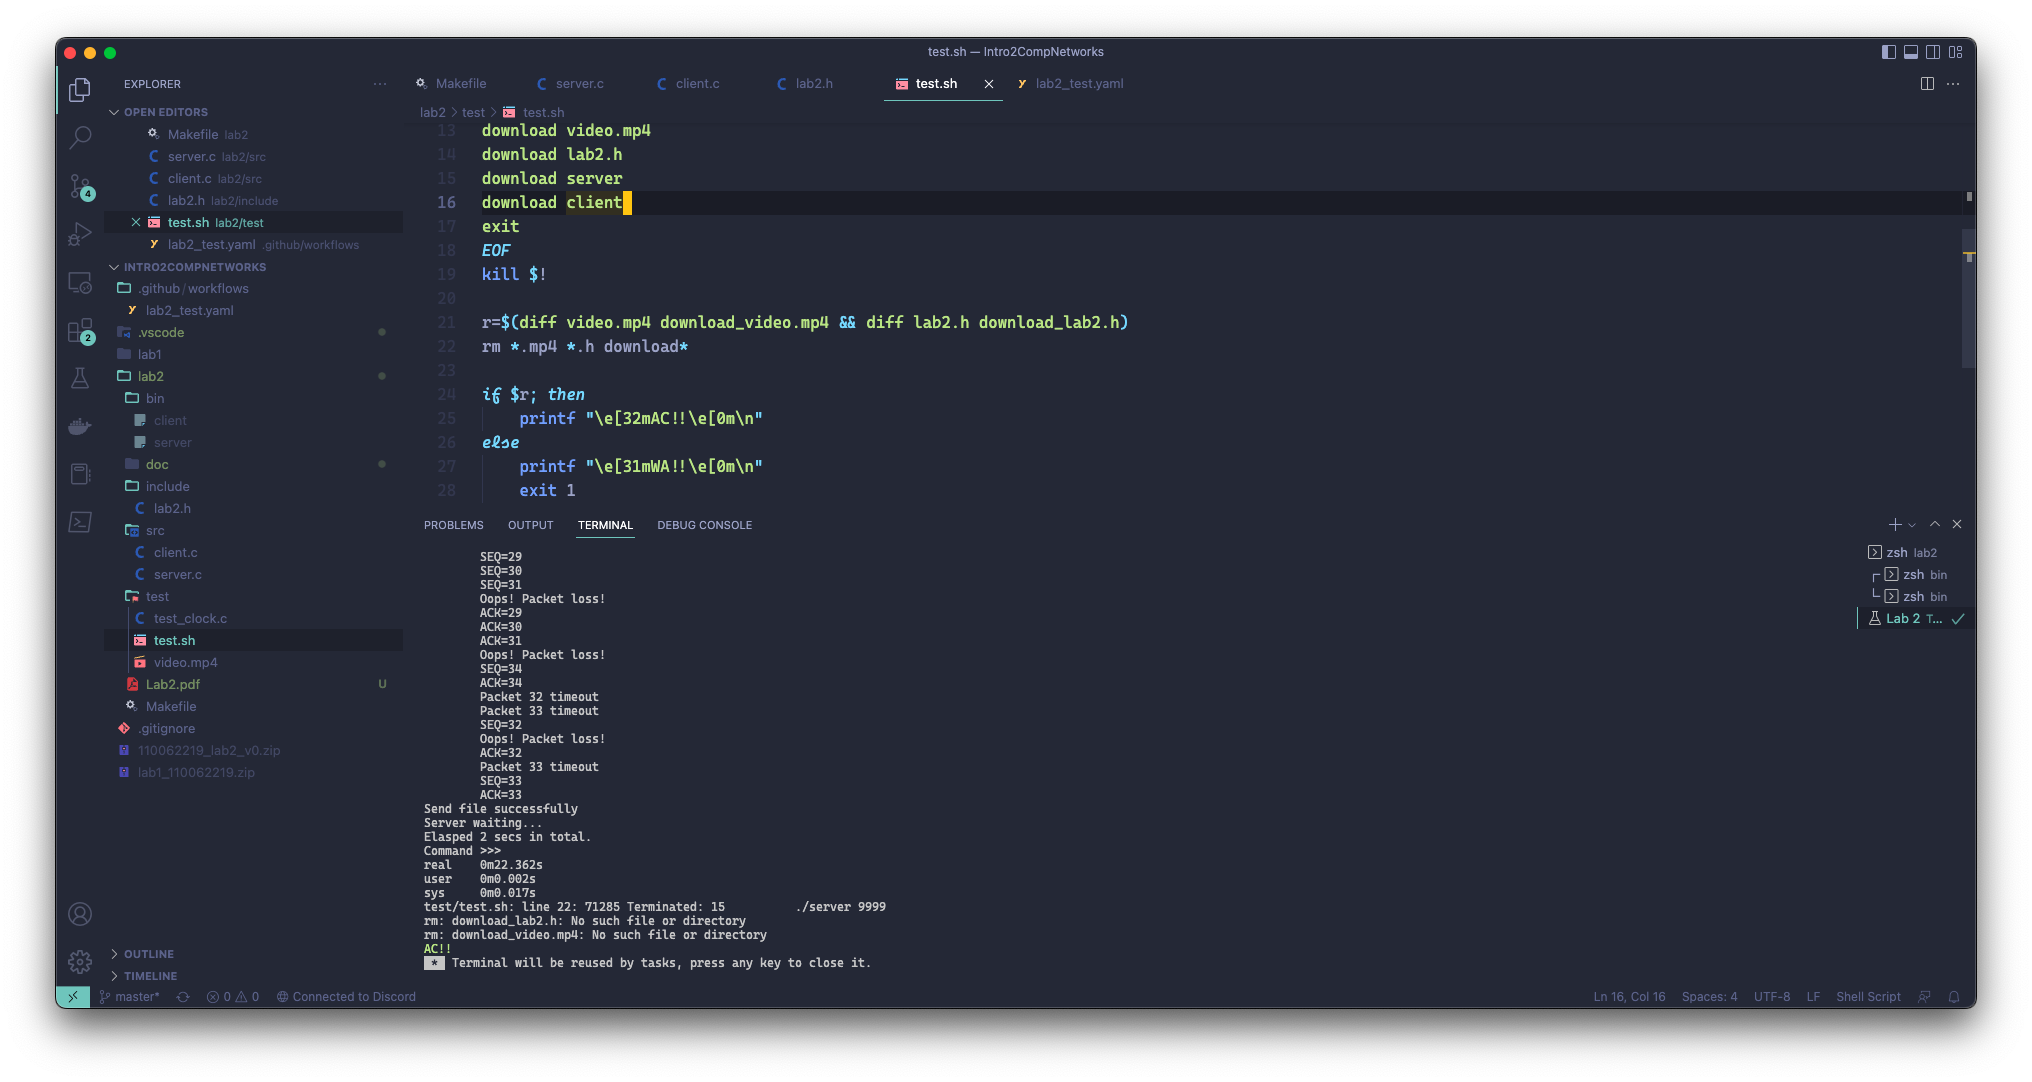
\includegraphics[width=\linewidth]{screenshot}
\caption{Screenshot of Bonus Tested on Local}
\label{fig:screenshot}
\end{figure}

\section{設計}

我有將助教提供的 code template 略作修改,包括一些輸出及錯誤處理的部分。為了利於偵錯,我將 client 模擬 packet loss 的機率寫成 Makefile 的變數,即可以透過 \texttt{make LOSS\_RATE=...} 以指定之,預設為 0.5.

\subsection{Server}

對於 selective repeat, server 的 \texttt{sendFile()} 除了原本的 main thread 以外,還需要另外兩個 thread 分別處理 ACK 的接收與 timeout.

Threads 間主要以 global variables 溝通,以 \texttt{mutex} 控制 sliding window base, timers and ACKed of each packet 的讀寫。

為了方便,我定義一個 function 來傳送 packet 並設定 timer.

\subsubsection{Main Thread}

傳送檔案前的準備有重設 global variables, 建立 threads 及將檔案讀入 buffer. 接著進入 loop, 當目前的封包落在 sliding window 中,則可以傳送,否則等待一下。

所有封包接傳送完第一次後,等待接受 ACK 的 thread 結束,停止 timeout thread 即完畢。

\subsubsection{ACK Reception Thread}

每當收到 ACK 時就加以記錄,若 sliding window base 已經被 ACKed 則不斷後移直到尚未被 ACKed, 或所有封包都被 ACKed 則結束。

\subsubsection{Timeout Thread}

這裡我是以一個無窮迴圈,不斷依序檢查所有封包的 timer, 如果 timeout 則重傳。

\subsection{Client}

Client 的部分就更簡單了。如果收到的封包超出 sliding window 則忽略。否則的話,寫入 buffer 並回覆 ACK. 對於最後一個封包,記錄其編號,當 sliding window base 超過時,則接收完畢。

\section{心得}

這次的 Lab 乍看之下似乎不太容易,不過實際寫起來又發現好像沒那麼難。當然,我還是有遇到一些錯誤跟困難。比如說,起初助教提供的 code template 遇到 packet loss 是直接 break, 我卻覺得應該是 continue 比較合理,但直到 Bonus 寫好我才發現應該要接收完之後再 continue 才回真的丟失封包。這時才發現 Basic 其實很有問題,因為 \texttt{recvfrom()} 是 blocking 的,我原本的寫法並不能正確 timeout. 這樣看來,Bonus 的 multithreading 反而還比較直觀。最後我是有以 \texttt{fd\_set}, \texttt{select()} 來完成 Basic.

此外,server code template 在開檔後 \texttt{fseek()} 至 EOF 再以 \texttt{ftell()} 得知檔案大小。一開始我不察,導致一直無法讀到檔案內容。不過,如果只是想要得知檔案大小,從頭 \texttt{fread()} 的回傳值即為所求,其實不必多次 \texttt{fseek()}. 跟檔案操作有關的還包括 client 我也曾忘記關檔,使得判斷是否成功下載時出現問題。

其他的一些小問題如無法連續下載、檔案如果小一點可能無法正確判斷 last..., 最後皆被一一克服。還有一些可以改進的地方,像是檢查 timeout 時我總是從第一個封包開始,其實我原本是想以一個 queue 維護等待被 ACKed 的封包及其 timer, 但是就有點懶得以 C 實作,畢竟目前版本也算是堪用,雖然重傳的順序不一定嚴格地理論上正確。

Socket programming 我覺得還滿有趣的,只做兩次 Lab 感覺是有點意猶未竟。雖然我自覺 codes 不是寫得很好看,尤其是變數命名得不是很好,畢竟需要遷就 code template, 但如果必須自己從頭開始大概也不容易。期中考的結果並不太令人滿意,這次 Lab Bonus 高達二十分,對我這種上課不太傾向於回答問題的學生真的是一大利多福音。原本以為計網概可能以 programming 為主,對於各種理論計算題實在不太習慣。系上研究所還有 \textsc{Computer Networks} 甚至是 \textsc{Advanced Computer Networks}, 不知道要不要修修看。

過往曾經以 Python, C++ 寫過 multithreading, 這是我首次以 C 使用 \texttt{pthread}. 對於平行程式我是很有興趣,可惜下學期同為 C 類專業必選修的 \textsc{Intro.~to Parallel Computing} 時間撞上必修的 \textsc{Software Studio}.

\subsection{CI/CD}

上次 Lab 就有提到手邊的 Intel 電腦硬碟容量不足,導致無法使用指定版本的 VM. 由於前陣子有嘗試 \LaTeX~自動編譯部署,這次我想到同樣可以利用 GitHub Actions 提供的服務,在指定版本的 Docker 容器化環境中,進行類似於 \textbf{CI/CD} \textit{(Continuous Integration / Continuous Deployment)} 的測試。

因此,我設計了自動測試、檢查的 shell script, 並整合至 Makefile. 但我有遇到一個小問題,就是在建置時 \texttt{pthread} 發生一些 undefined reference 的錯誤。進一步檢查,助教所提供的 Makefile \texttt{\$(CC)  \$< -o \$@ -lm -lpthread} 在我自己的 M1 Mac mini w/ Apple clang 或國網中心 Taiwania 3 w/ GCC 9.4.0 皆沒有問題,在討論區詢問後助教在 VM 或一般的 Docker 也都無法重現。

雖然整起問題感覺很弔詭,比如 Ubuntu 20.04 內建的 GCC 應該是 9.3.0, 但 GitHub Actions 的容器卻是 9.4.0. 不過,總之我上網查到到編譯時 \texttt{CLFAGS} 加上 \texttt{-pthread} 後,就可以順利編譯。然而,我還是不太明白,\texttt{-lpthread}, \texttt{-pthread} 這兩個 options / flags 分別的用途為何,又該在什麼場景使用。

\begin{figure}
\centering
\begin{subfigure}{\linewidth}
\centering
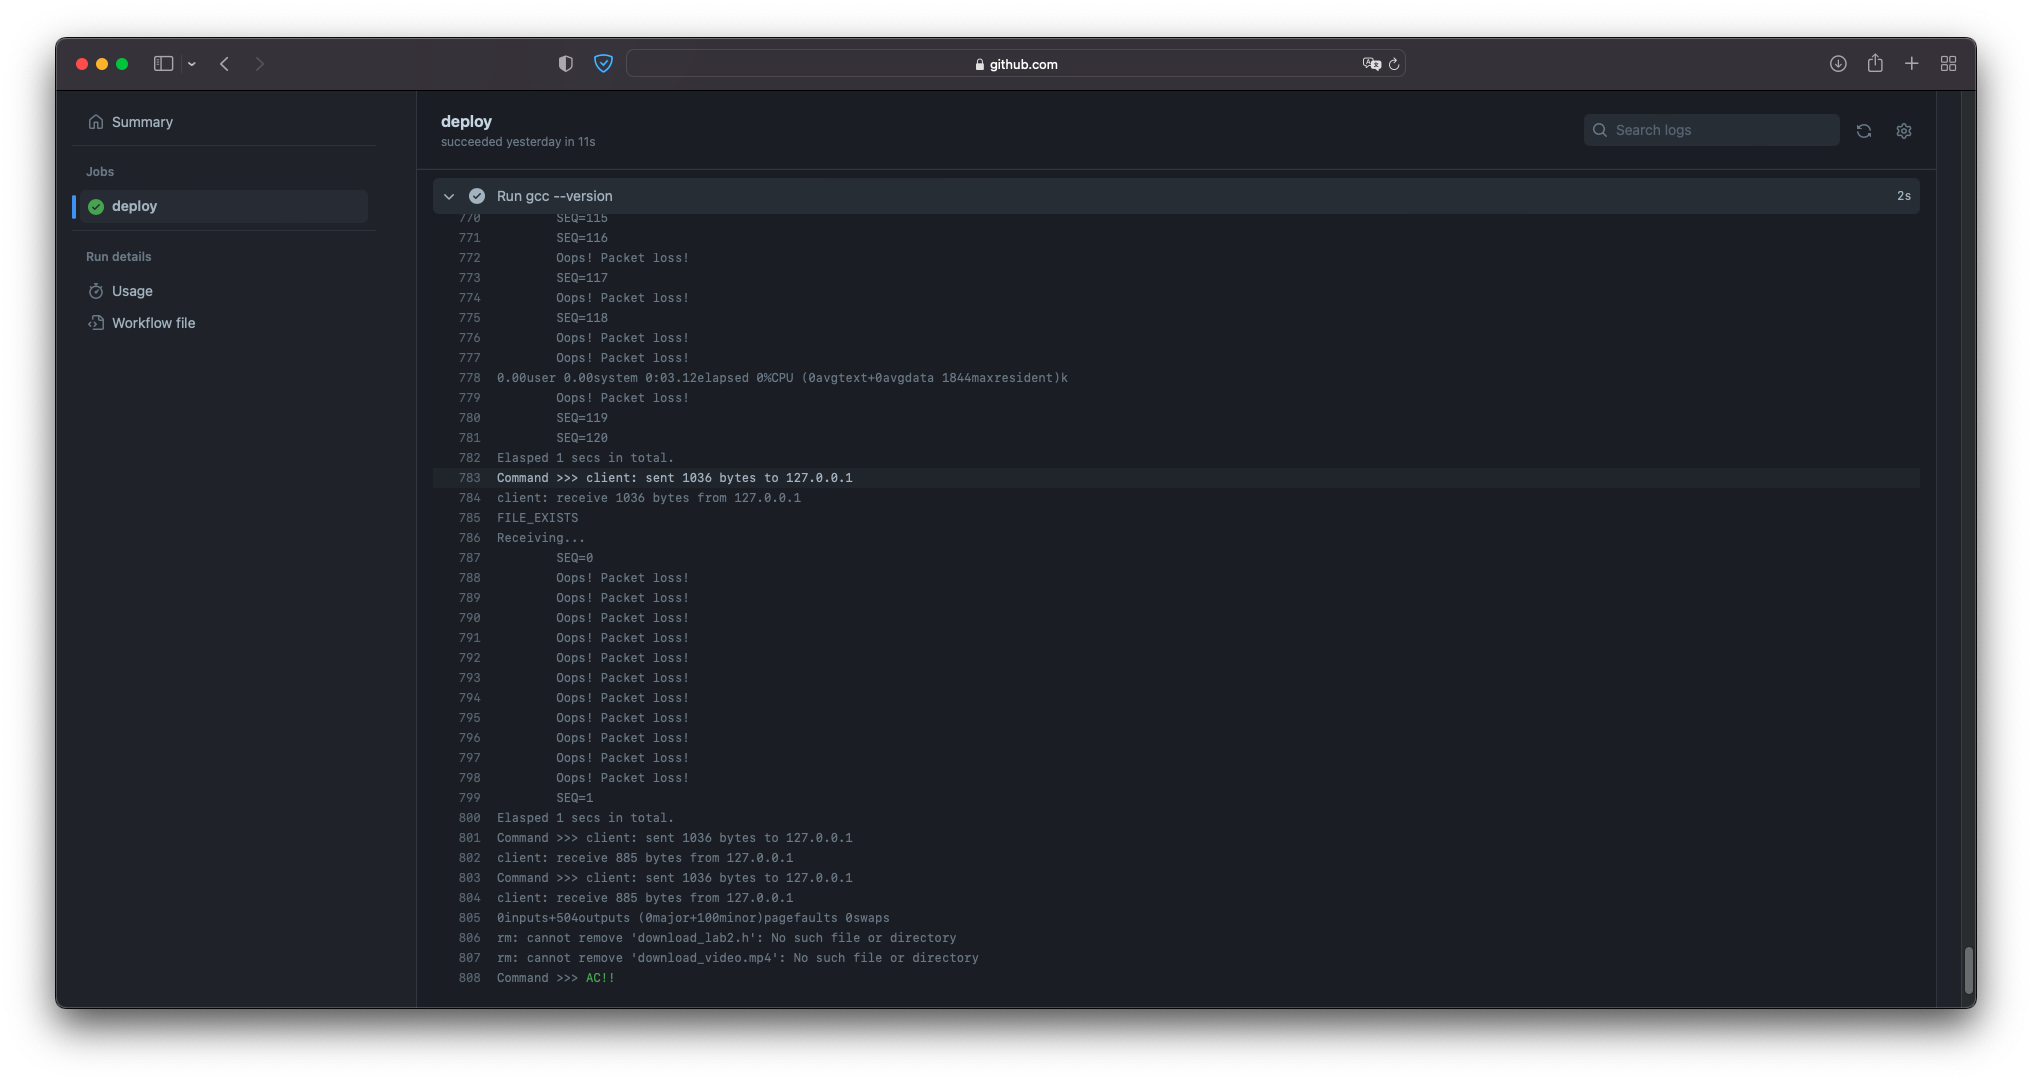
\includegraphics[width=\linewidth]{ci-cd_basic}
\caption{Test of Basic}
\label{fig:ci-cd_basic}
\end{subfigure}
\begin{subfigure}{\linewidth}
\centering
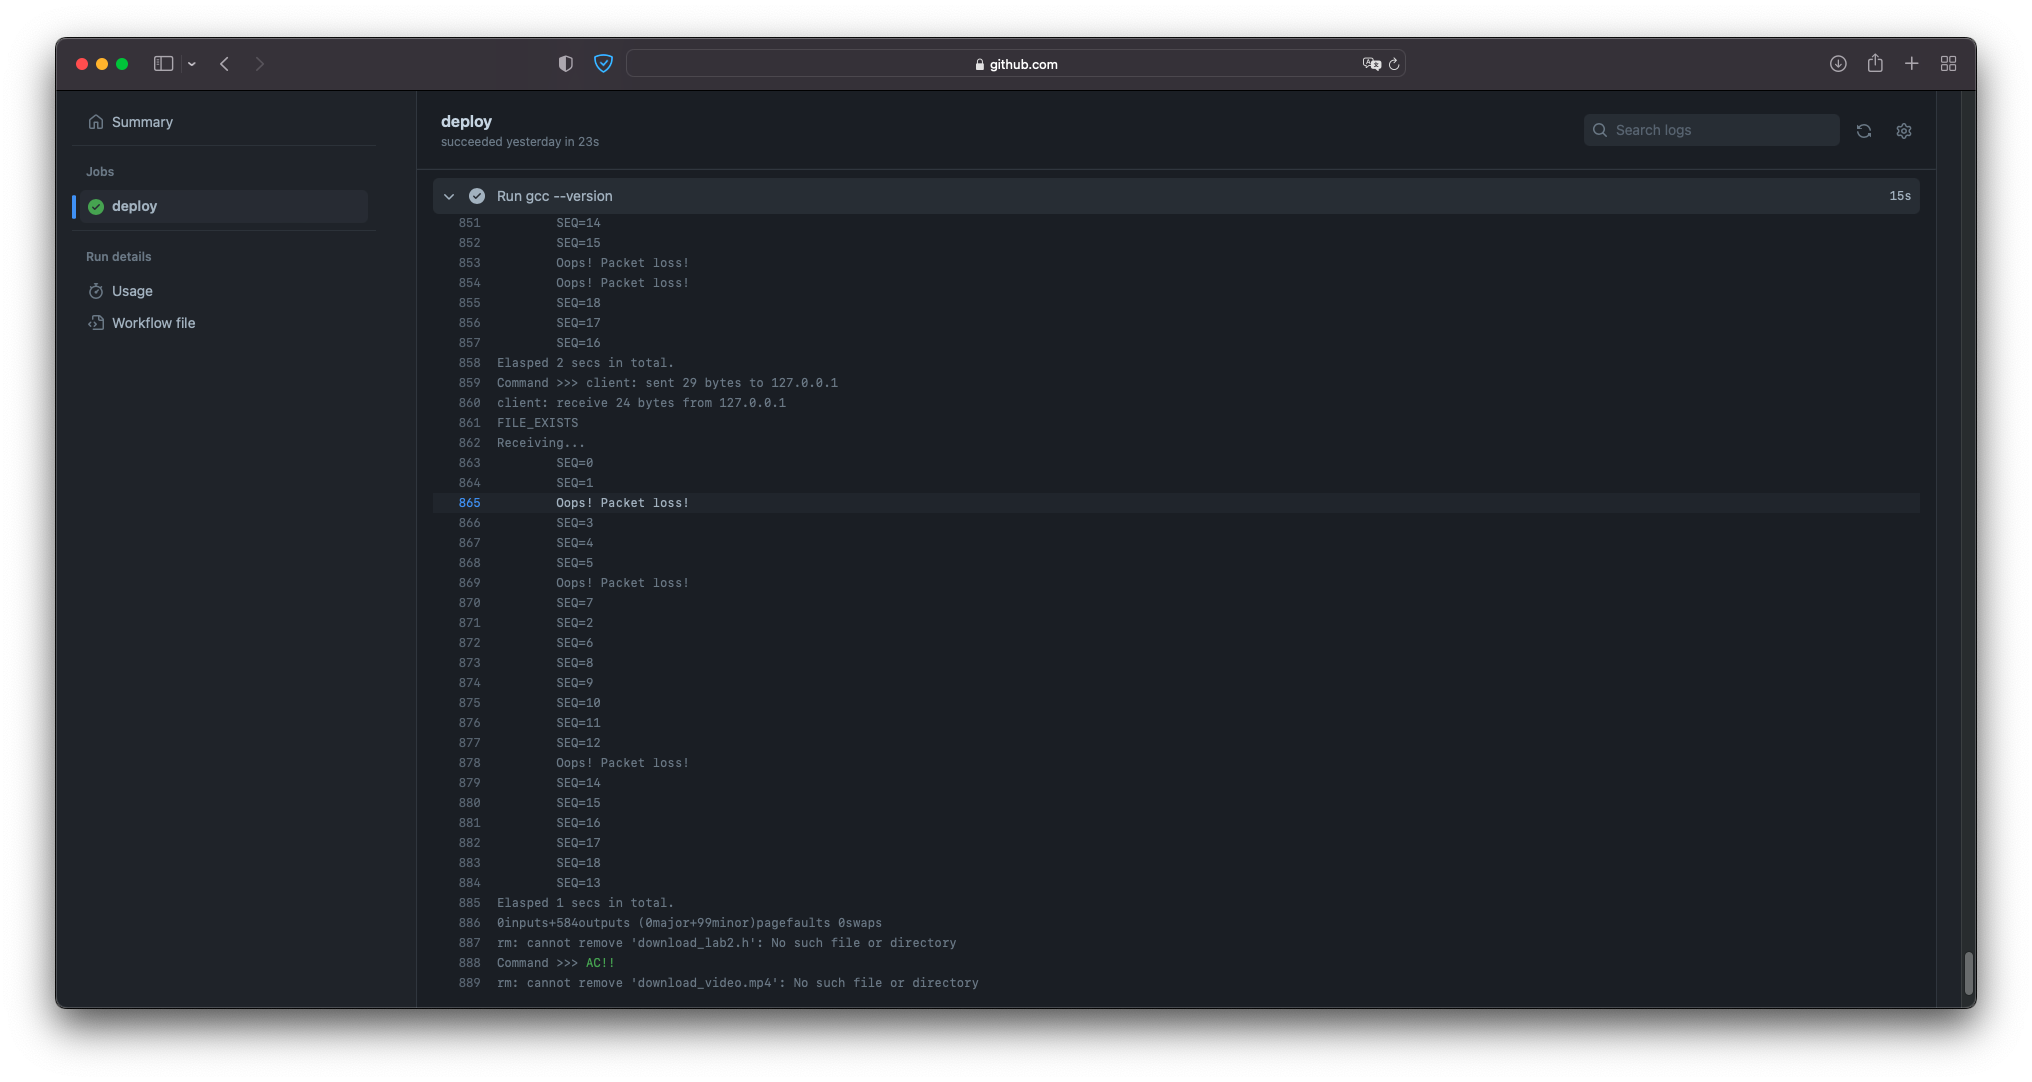
\includegraphics[width=\linewidth]{ci-cd_bonus}
\caption{Test of Bonus}
\label{fig:ci-cd_bonus}
\end{subfigure}
\caption{CI/CD by GitHub Actions}
\end{figure}

\begin{table}[htp]
\caption{Testbed (in Test Order)}
\centering
\begin{tabular}{c|c|c|c}
OS & Arch. & Compiler & Note \\\hline
%Ubuntu 18.04 & x86-64 & GCC 10 & WSL 2 \\
macOS 12.4 & AArch64 & Apple clang 13.1.6 \\
Ubuntu 20.04 & x86-64 & GCC 9.4.0 & Docker\footnotemark \\
CentOS 7.8 & x86-64 & GCC 9.4.0 \\
macOS 11.6.4 & x86-64 & Apple clang 12.0.5 \\
Ubuntu 22.04 & x86-64 & GCC 11.2.0 & VM \\
\end{tabular}
\label{tab:testbed}
\end{table}

\pagebreak[4]
\footnotetext{GitHub Action}

\section*{Acknowledgements}

I thank to \textsf{National Center for High-performance Computing} \textit{(NCHC)} for providing computational and storage resources.

\end{document}
